\documentclass[a4paper,14pt]{article}
\usepackage{float}
\usepackage{extsizes}
\usepackage{amsmath}
\usepackage{amssymb}
\everymath{\displaystyle}
\usepackage{geometry}
\usepackage{fancyhdr}
\usepackage{multicol}
\usepackage{graphicx}
\usepackage[brazil]{babel}
\usepackage[shortlabels]{enumitem}
\usepackage{cancel}
\usepackage{textcomp}
\columnsep=2cm
\hoffset=0cm
\textwidth=8cm
\setlength{\columnseprule}{.1pt}
\setlength{\columnsep}{2cm}
\renewcommand{\headrulewidth}{0pt}
\geometry{top=1in, bottom=1in, left=0.7in, right=0.5in}

\pagestyle{fancy}
\fancyhf{}
\fancyfoot[C]{\thepage}

\begin{document}
	
	\noindent\textbf{8FMA74 - Matemática} 
	
	\begin{center}Gráficos de relações dadas por mais de uma sentença (Versão estudante)
	\end{center}
	
	\noindent\textbf{Nome:} \underline{\hspace{10cm}}
	\noindent\textbf{Data:} \underline{\hspace{4cm}}
	
	%\section*{Questões de Matemática}
	
	
    \begin{multicols}{2}
    	\noindent Quando mais de uma sentença define a relação entre $x$ e $y$, fazemos os gráficos referentes às sentenças observando as restrições de cada variável.
    	\noindent\textsubscript{~---------------------------------------------------------------------------}
		\begin{enumerate}
			\item Faça o gráfico de:
			\begin{enumerate}[a)]
				\item $y =
				\begin{cases}
					3x+4, \text{se~} x \leq 0 \\
					-x + 4, \text{se~} x > 0
				\end{cases}$\\\\\\\\\\\\\\\\\\\\
			    \item $x = 
			    \begin{cases}
			    	y - 5, \text{se~} y > 1 \\
			    	-y + 1, \text{se~} y < 1
			    \end{cases}$\\\\\\\\\\\\\\\\\\\\
			\end{enumerate}
		    \item Qual a área da região delimitada pelo gráfico de \\ $|x| + |y| = 2$?\\
		    Sugestão: use o fato de que $|a| = \begin{cases} 
		    	a, \text{se~} a \geq 0 \\
		    	-a, \text{se~} a < 0
		    	\end{cases}$\\\\\\\\\\\\\\\\\\\\
	    	\item Determine $p$ para que o gráfico a seguir seja o da relação:\\
	    	$x = \begin{cases}
	    		-\frac{4p^2}{3}y + p + 9, \text{se~} y > 0 \\
	    		-\frac{8p}{5} + p^2 + 7, \text{se~} y \leq 0
	    	\end{cases}$
    	    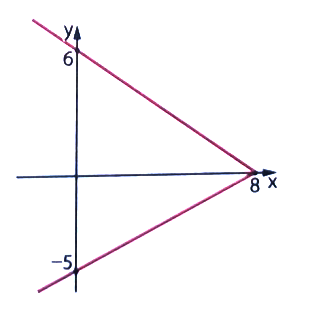
\includegraphics[width=1\linewidth]{imagens_8FMA74/imagem1}
    	    \newpage
        \end{enumerate}
    \end{multicols}
    	    \noindent\textbf{Desafio olímpico}\\\\
    	    (OBMEP) Duas formiguinhas partiram ao mesmo tempo e em direções diferentes de um mesmo vértice de um triângulo equilátero de lado 2 cm. Elas andaram sobre os lados do triângulo à velocidade de 1 cm/s, até retornar ao vértice inicial. \\
    	    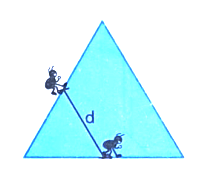
\includegraphics[width=0.3\linewidth]{imagens_8FMA74/imagem2}\\
    	    Qual dos gráficos abaixo descreve a distância $d$ entre as duas formiguinhas em função do tempo? \\
    	    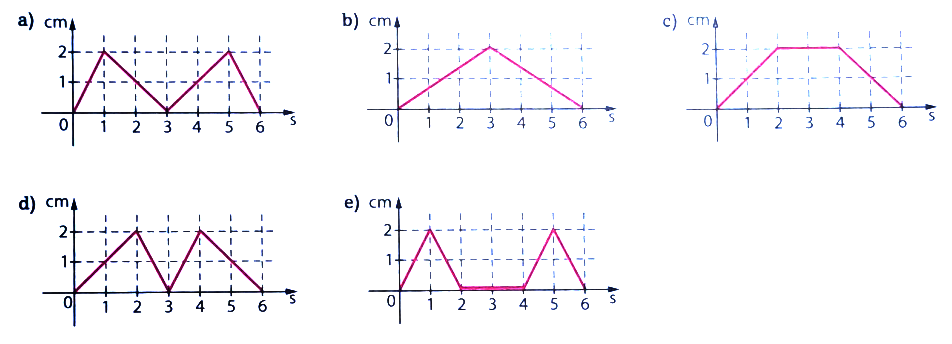
\includegraphics[width=1\linewidth]{imagens_8FMA74/imagem3}
    	    \newpage
    \begin{multicols}{2}
    	\begin{enumerate}
    	    \item Faça os gráficos abaixo utilizando tabelas e, para os itens $a$ e $b$, faça também no GeoGebra.
    	    \begin{enumerate}[a)]
    	    	\item $y =
    	    	\begin{cases}
    	    		x + 5, \text{se~} x \leq -1 \\
    	    		-3x + 2, \text{se~} x > -1
    	    	\end{cases}$\\\\\\\\\\\\\\\\\\\\
    	    	\item $y = 
    	    	\begin{cases}
    	    		x^2 - 2, \text{se~} x \geq 0 \\
    	    		-x^2 - 2, \text{se~} x < 0
    	    	\end{cases}$\\\\\\\\\\\\\\\\\\\\
	        	\item $y = 
	        	\begin{cases}
	        		-3, \text{se~} x < -2 \\
	        		\frac{5}{3}x + \frac{1}{3}, \text{se~} -2 \leq x \leq 1 \\
	        		-x + 3, \text{se~} x > 1
	        	\end{cases}$\\\\\\\\\\\\\\\\\\\\
    	    \end{enumerate}
            \item (Enem) Certo vendedor tem seu salário mensal calculado da seguinte maneira: ele ganha um valor fixo de R\$ 750,00, mais uma comissão de R\$ 3,00 para cada produto vendido. Caso ele venda mais de 100 produtos, sua comissão passa a ser de R\$ 9,00 para cada produto vendido, a partir do $1\textsuperscript{º}$ produto vendido. Com essas informações, o gráfico que melhor representa a relação entre salário e o número de produtos vendidos é:
            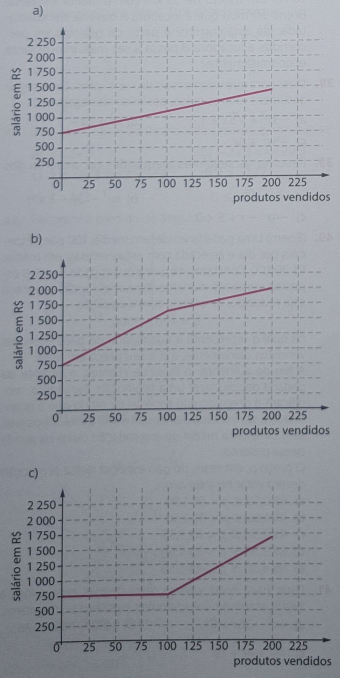
\includegraphics[width=1\linewidth]{imagens_8FMA74/imagem4}
            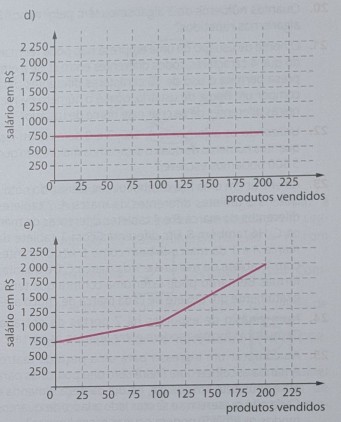
\includegraphics[width=1\linewidth]{imagens_8FMA74/imagem5}
        \end{enumerate}
    $~$ \\ $~$ \\ $~$ \\ $~$ \\ $~$ \\ $~$ \\ $~$ \\ $~$ \\ $~$ \\ $~$ \\ $~$ \\ $~$ \\ $~$ \\ $~$ \\ $~$ \\ $~$ \\ $~$ \\ $~$ \\ $~$ \\ $~$ \\ $~$ \\ $~$ \\ $~$ \\ $~$ \\ $~$ \\ $~$ \\ $~$ \\ $~$ \\ $~$ \\ $~$ \\ $~$ \\ $~$ \\ $~$ \\ $~$ \\ $~$ \\ $~$ \\ $~$ \\ $~$ \\ $~$ \\ $~$ \\ $~$ \\ $~$ \\ $~$ \\ $~$ \\ $~$ \\ $~$ \\ $~$ \\ $~$ \\ $~$ \\ $~$ \\ $~$ \\ $~$ \\ $~$ \\ $~$ \\ $~$ \\ $~$ \\ $~$ \\ $~$ \\ $~$ \\ $~$ \\ $~$ \\ $~$ \\ $~$ \\ $~$ \\ $~$ \\ $~$ \\ $~$ \\ 
    \end{multicols}
\end{document}